\section{Related Work}
% Sec 2.1. Review of previous work (i.e. previous methods that have explored a similar problem)
% Sec 2.2. Say why your method is better than previous work; and/or summarize the key main contributions of your work;
\subsection{StyleGAN}
When it comes to generating images from style aware latent codes, StyleGAN-based work must first come to our mind. There are several styleGAN based works, such as original styleGAN \cite{karras2019style} and styleGAN2 \cite{karras2020analyzing}. These works focus on diversity and quality on the generated images. However, the ultimate goal of these works is using random latent code to generate diverse and plausible images, while our goal is to use specific latent code to reconstruct the same images and apply latent code interpolation to mix the style of two given faces, which is totally different from original styleGAN based works.

To address this issue, we finally find some similar works called style encoding. Style encoding generates corresponding latent codes based on input images. We find two works focusing on style encoding tasks \cite{karras2020training} \cite{richardson2021encoding}. Finally we decide the latter one because its style encoder outperforms the former one. 

\subsection{Human Pose}
There are many existing work focusing on human pose estimation, such as YOLO \cite{yolo1} \cite{wang2022yolov7} \cite{yolo3}. However, we find that if we inference on our laptop, it'll run very slow. The FPS of the game will drop to 2 or 3, which is unsuitable for our application. What we need is a simple backbone that can perform human pose estimation real-time, instead of a heavy backbone that can predict very accurately.

Therefore, we search for a simple network that satisfies our goal, \textbf{mediapipe}~\cite{lugaresi2019mediapipe}. We find that it can perform human pose estimation in real-time, mainly due to two reasons. First, Figure~\ref{fig:yolo_arch} and Figure~\ref{fig:mp_arch} shows the architecture of YOLOv7~\cite{wang2022yolov7} and mediapipe respectively. We can easily find that the architecture of YOLOv7~\cite{wang2022yolov7} is far more complicated than that of mediapipe~\cite{lugaresi2019mediapipe}, which implies that the number of parameters in mediapipe~\cite{lugaresi2019mediapipe} is far less than that in YOLOv7~\cite{lugaresi2019mediapipe}, so the inference speed will be faster.

\begin{figure}[ht]
    \centering
    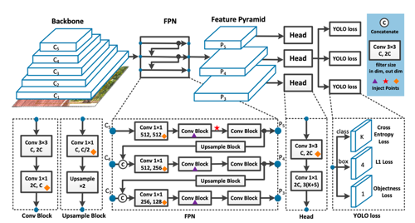
\includegraphics[scale=.6]{fig/yolo_arch.png}
    \caption{Architecture of YOLOv7 \cite{wang2022yolov7}.}
    \label{fig:yolo_arch}
\end{figure}

\begin{figure}[ht]
    \centering
    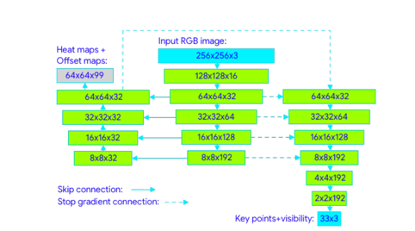
\includegraphics[scale=.6]{fig/mp_arch.png}
    \caption{Architecture of Mediapipe \cite{lugaresi2019mediapipe}.}
    \label{fig:mp_arch}
\end{figure}

Second, unlike most human pose backbones that perform detection at every single frame, mediapipe only performs human detection at the very beginning frame as Figure \ref{fig:mp_det} shows. This approach greatly reduces the computational cost. Combined with 2 advantages mentioned above, mediapipe seems to be the best choice for our application.

\begin{figure}[ht]
    \centering
    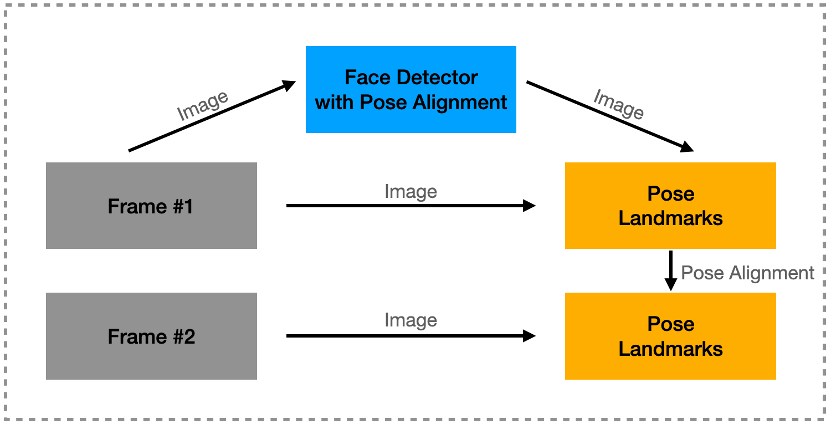
\includegraphics[scale=.5]{fig/mp_det.png}
    \caption{Mediapipe only performs human detection at the very beginning frame, which greatly reduces the computational cost.}
    \label{fig:mp_det}
\end{figure}

The original version of mediapipe, however, only supports human pose estimation for single person, but our game definitely requires the simultaneous huamn pose estimation on two people. Therefore, we make some modifications to it, which will be elaborated in Section \ref{mediapipework}.